\documentclass{article}

\usepackage[dblblindworkshop,final]{neurips_2026}
\usepackage[utf8]{inputenc}
\usepackage[T1]{fontenc}
\usepackage{hyperref}
\usepackage{url}
\usepackage{booktabs}
\usepackage{amsfonts}
\usepackage{amsmath}
\usepackage{amssymb}
\usepackage{nicefrac}
\usepackage{microtype}
\usepackage[table]{xcolor}
\usepackage{array}
\usepackage{graphicx}

\title{Consistency Is Not Enough: From Routing Stability to Compositional Robustness in Mixture-of-Experts}
\workshoptitle{NeurIPS 2026 Workshop on Efficient Systems for Foundation Models}

\author{
  \textbf{Diego Calanzone}$^{1}$ \quad \textbf{Riyasat Ohib}$^{2}$ \quad \textbf{Pierre-Luc Bacon}$^{1,3}$ \\[0.3em]
  \small $^{1}$Mila, Quebec AI Institute \quad
  $^{2}$Georgia Institute of Technology \quad
  $^{3}$Universit\'e de Montr\'eal \\
  \small \texttt{diego.calanzone@mila.quebec}, \texttt{PLACEHOLDER@gatech.edu}, \texttt{PLACEHOLDER@umontreal.ca}
}

\begin{document}
\maketitle

\begin{abstract}
Fine-tuning a mixture-of-experts (MoE) router to reuse a stable set of experts across a
sequence is usually motivated as a serving-efficiency trick, but stable routing is only
useful insofar as it reflects something deeper: that individual experts specialize into
reusable, semantically coherent modules, and that this modularity in turn makes the
model's behavior more robust when its input changes. We make this chain explicit with
CAR-MoE (Cache-Aware Routing for MoE), a GRPO-trained router objective that rewards a
simulated working-set hit ratio. On two backbones (Phi-tiny-MoE-instruct, OLMoE-1B-7B)
and five objectives (base, supervised fine-tuning, CAR-MoE, an option-critic-style
controller, and MELINOE), we measure benchmark performance and robustness to input
perturbation, working-set hit ratio and cache misses, and routing \emph{consistency} and
\emph{modularity} via a specialization index. CAR-MoE is the most robust objective tested
on both backbones, improving hit ratio and benchmark retention alongside robustness
rather than trading one off against another. An option-critic-style controller, in
contrast, reaches near-perfect routing consistency, the highest specialization score, and
a perfect hit ratio, by collapsing its routing onto a handful of experts, and this
degenerate profile coincides with the \emph{worst} robustness in the comparison.
Stability, we conclude, is necessary but not sufficient evidence of useful modularity: it
must be checked against routing diversity and downstream robustness directly, not
assumed.
\end{abstract}

\section{Introduction}

A mixture-of-experts router fine-tuned to reuse a small, stable set of experts per
sequence is typically justified purely as a memory-traffic optimization. But routing
consistency, on its own, is not obviously a virtue: a router that always activates the
same expert regardless of input is maximally consistent and maximally useless. What
should actually matter is \emph{modularity}, i.e., whether individual experts specialize
into coherent, reusable functional units, so a consistent routing decision reflects a
genuine correspondence between content and expert identity rather than an arbitrary or
collapsed assignment. And modularity should matter only because it is the mechanism by
which a model \emph{composes} its specialized parts robustly when its environment
changes, e.g., when the same task is presented under surface noise, paraphrase, or
distribution shift.

This paper makes that three-step chain, consistency for modularity for robustness to a
changing environment, explicit, and measures each link directly rather than treating
routing consistency as a terminal objective. We build on CAR-MoE (Cache-Aware Routing for
MoE), which fine-tunes a router with GRPO against a stateful reward simulating a
fixed-capacity LRU cache of experts, so that the policy is rewarded for sequence-level
expert reuse without any custom auxiliary loss or architectural change to the routing
mechanism (Section~\ref{sec:method}). We compare it against a plain base model,
supervised fine-tuning (SFT) alone, an option-critic-style temporally extended controller
\citep{shen2026temporal,bacon2017optioncritic}, and MELINOE \citep{raje2026melinoe}, on
two backbones of different scale, and ask, for each: does it improve downstream task
performance and robustness to input perturbation; does it improve working-set efficiency;
and is its routing consistent and its experts specialized by content domain. The answer
is not uniformly yes, and the exception is informative: an objective can appear maximally
consistent, modular, and cache-efficient by every aggregate statistic while being the
least robust of the comparison, because it achieves that appearance through routing
collapse rather than genuine specialization.

\section{Method}
\label{sec:method}

\subsection{CAR-MoE: Cache-Aware Routing for MoE}

We simulate a fixed-capacity LRU cache of experts at one middle transformer layer,
treating each token's top-$K$ expert request as a cache access. Let $p_t \in \Delta^E$ be
the router's distribution over $E$ experts at token $t$, $e_t = \mathrm{TopK}(p_t, K)$ the
set of experts requested at that token, and $\mathcal{C}_{t^-} \subseteq \{1,\dots,E\}$,
$|\mathcal{C}_{t^-}| \le c$, the set of experts resident in the cache immediately before
token $t$, for a target capacity $c$. For each requested $e \in e_t$: if $e \in
\mathcal{C}_{t^-}$, the access is a hit and $e$ is promoted to most-recently-used;
otherwise it is a miss, $e$ is inserted, and the least-recently-used resident expert is
evicted once capacity is exceeded. At training time we route densely, i.e., every expert
participates in the forward pass weighted by $p_t$, and reward the policy with the
probability mass the cache already holds before the update, a soft relaxation of the hit
indicator requiring no discrete cache simulation on the backward pass:
\begin{equation}
  r_t = \sum_{e \in \mathcal{C}_{t^-}} p_t[e],
  \qquad
  R(x,y) = \frac{1}{T}\sum_{t=1}^{T} r_t,
  \label{eq:reward}
\end{equation}
with $T$ the number of generated tokens and $R(x,y)$ the sequence-level reward handed to
GRPO/DAPO \citep{shao2024deepseekmath,yu2025dapo}. This reward is stateful, since the
value at token $t$ depends on the entire cache trajectory up to that point, but requires
no additional trainable parameters and no architectural change to the router. At
evaluation time we replace the soft reward with its hard counterpart via deterministic
top-$K$ routing; the working-set hit ratio of a rollout is the fraction of requested
experts already resident, and misses are counted over the whole sequence.

Every objective, baselines included, is trained as a LoRA adapter over the frozen
backbone, so absolute downstream scores are somewhat lower than a full fine-tune would
reach, uniformly across methods. We therefore report benchmark performance as $\Delta$
from each backbone's own base model (Table~\ref{tab:main}), alongside the working-set hit
ratio and mean cache misses from the same simulated cache CAR-MoE is trained against.
Full training, dataset, and backbone details are given in
Appendix~\ref{app:setup}.

\subsection{Consistency, Modularity, and Robustness Metrics}

\paragraph{Consistency.} For a held-out prompt, we take a teacher-forced forward pass and
pool the top-1 expert choice over all valid tokens into a per-expert usage histogram. We
build two meaning-preserving perturbed copies of each prompt: character-level typo noise
and cosmetic case and whitespace noise (details in Appendix~\ref{app:setup}). We measure
consistency as the Jensen-Shannon divergence \citep{lin1991divergence} between the
original and perturbed histograms, averaged over held-out prompts; lower divergence means
the router's aggregate expert usage is invariant to surface form.

\paragraph{Modularity.} Following work on functional modularity in neural networks
\citep{csordas2021modular}, we ask whether individual experts specialize to a fixed
content domain rather than routing uniformly regardless of it. We sample two
disjoint-domain prompt pools (math and code, from the Nemotron Post-Training Dataset v2,
\citealp{nvidia2025nemotron}) and compute each expert's domain-conditional usage
$P(\text{math} \mid e) = n_{\text{math}}(e) / (n_{\text{math}}(e) + n_{\text{code}}(e))$
from pooled usage counts. An expert's specialization index is $|P(\text{math}\mid e) -
0.5| \times 2 \in [0,1]$; we report the mean specialization and the fraction of experts
with specialization above $0.6$. Good modularity should show up as invariance to the
surface noise above and sensitivity to this genuine domain shift, the complement of the
consistency measure.

\paragraph{Robustness.} We adopt the character-level perturbation used to test sequence
models' robustness to natural noise \citep{belinkov2018synthetic} and measure the
resulting drop in exact-match accuracy on GSM8K as our robustness measure, so the same
kind of perturbation grounds both the consistency measure and this downstream check. The
evaluation protocol (four-shot exemplars, answer extraction, held-out question count) is
given in Appendix~\ref{app:setup}.

\section{Results}

\begin{table}[h]
\centering
\scriptsize
\caption{Benchmark performance, working-set efficiency, routing consistency,
modularity, and robustness for every (backbone, objective) combination, at each
backbone's trained working-set capacity (Phi: $c=4$; OLMoE: $c=16$; Appendix~\ref{app:setup}).
Avg~$\Delta$Bench: mean $\Delta$ from the backbone's own base model over MMLU, MMMLU,
GSM8K, HumanEval, and MATH (positive is better). Hit ratio / Misses: working-set hit ratio
and mean misses per sequence (higher hit ratio / lower misses is better). JS-typo/JS-fmt:
Jensen-Shannon divergence between original and perturbed routing histograms (lower is more
consistent). Spec.-frac: fraction of experts with specialization $>0.6$ (higher is more
modular). $\Delta$Acc: GSM8K accuracy drop under typo perturbation (lower is more
robust). CAR-MoE rows highlighted; the option-critic controller's row is marked
$\dagger$ and discussed in Section~\ref{sec:consistency-results}.}
\renewcommand{\arraystretch}{0.9}
\resizebox{\textwidth}{!}{%
\begin{tabular}{ll ccc ccc c}
\toprule
Backbone & Objective & Avg~$\Delta$Bench & Hit ratio & Misses & JS-typo & JS-fmt & Spec.-frac & $\Delta$Acc \\
\midrule
Phi-tiny-MoE & Base (untuned)  & --      & 0.571 & 649.8 & 0.055 & 0.014 & 0.25 & 0.233 \\
Phi-tiny-MoE & SFT             & $-$0.01 & 0.565 & 742.1 & 0.053 & 0.014 & 0.25 & 0.247 \\
\rowcolor{black!8}
Phi-tiny-MoE & CAR-MoE         & $-$0.01 & 0.622 & 435.9 & 0.054 & 0.015 & 0.25 & \textbf{0.220} \\
Phi-tiny-MoE & Option-critic$^\dagger$ & $-$0.05 & \textbf{1.000} & \textbf{0.1} & 0.0001 & 0.00003 & \textbf{0.94} & 0.287 \\
Phi-tiny-MoE & MELINOE         & $-$0.05 & 0.879 & 237.7 & 0.046 & 0.011 & 0.44 & 0.333 \\
\midrule
OLMoE-1B-7B  & Base (untuned)  & --      & 0.686 & 1874.2 & 0.096 & 0.031 & 0.53 & 0.080 \\
OLMoE-1B-7B  & SFT             & $-$0.05 & 0.679 & 1943.9 & 0.095 & 0.031 & 0.56 & 0.233 \\
\rowcolor{black!8}
OLMoE-1B-7B  & CAR-MoE         & $+$0.01 & \textbf{0.759} & \textbf{1004.2} & 0.094 & 0.030 & 0.52 & \textbf{0.073} \\
OLMoE-1B-7B  & Option-critic   & $-$0.11 & 0.684 & 2012.7 & 0.100 & 0.033 & 0.58 & 0.167 \\
OLMoE-1B-7B  & MELINOE         & $-$0.14 & 0.763 & 1541.9 & 0.081 & 0.026 & 0.55 & 0.173 \\
\bottomrule
\end{tabular}%
}
\label{tab:main}
\end{table}

\subsection{Benchmark performance and downstream robustness}

CAR-MoE achieves the smallest GSM8K accuracy drop of any objective tested, on
\emph{both} backbones: 0.073 on OLMoE-1B-7B, versus 0.080 base and 0.233 SFT (a
$3.2\times$ larger drop), and 0.220 on Phi-tiny-MoE, versus 0.233 base, 0.247 SFT, and
0.333 MELINOE. On OLMoE-1B-7B, CAR-MoE also loses the least average benchmark score of
any fine-tuned objective ($-$0.01, versus $-$0.05 SFT, $-$0.11 option-critic, $-$0.14
MELINOE), so its accuracy-drop advantage is not bought with a larger sacrifice on
ordinary task performance. Standard benchmark performance and robustness to input
perturbation thus move together across objectives rather than trading off, and CAR-MoE
sits at the favorable end of both on every backbone tested; option-critic and MELINOE are
instead the two weakest objectives on both fronts.

\subsection{Working-set efficiency: hit ratio and cache misses}

CAR-MoE also raises the working-set hit ratio the most of any non-collapsed objective on
both backbones: 0.759 versus 0.686 base on OLMoE-1B-7B, a 46\% cut in mean misses per
sequence (1004.2 versus 1874.2), and 0.622 versus 0.571 base on Phi-tiny-MoE (misses 435.9
versus 649.8). Efficiency, benchmark retention, and robustness therefore improve together
under CAR-MoE rather than trading off against one another. The option-critic controller
reaches a strictly higher hit ratio than CAR-MoE on Phi-tiny-MoE, in fact the highest
possible value (1.000, at 0.1 mean misses versus hundreds for every other objective), which
by this statistic alone would look like the best outcome for the underlying
serving-efficiency motivation. Section~\ref{sec:consistency-results} shows why that
reading is misleading.

\subsection{Consistency, modularity, and the collapse behind a perfect hit ratio}
\label{sec:consistency-results}
\label{sec:discussion}

Figure~\ref{fig:scatter} plots consistency and modularity against the robustness measure
directly. Within each backbone, CAR-MoE and the base/SFT objectives cluster together on
both axes: its JS-typo, JS-fmt, and specialization numbers sit within noise of base and
SFT (Table~\ref{tab:main}), so CAR-MoE reaches the efficiency and robustness gains above
through genuine, non-collapsing reuse of an already-reasonable routing policy, not a
change in how the router treats its input.

Phi-tiny-MoE's option-critic controller is the clear outlier in Figure~\ref{fig:scatter}
and breaks this pattern sharply. Its routing consistency is roughly three orders of
magnitude better than every other objective (JS-typo $\approx 0.0001$ versus $0.05$ to
$0.10$ elsewhere), and its specialization fraction (0.94) is the highest of any
objective, alongside the perfect hit ratio already noted above. By every aggregate
statistic this looks like the clearest success case for the whole story, yet it is the
\emph{least} robust objective tested ($\Delta$Acc $=0.287$) and among the weakest on
benchmark score. A routing trace analysis (Appendix~\ref{app:trace}, Figure~\ref{fig:trace})
explains the discrepancy: the controller collapses onto a small, fixed subset of experts
resident for essentially the whole sequence rather than tracking content, so the perfect
hit ratio is a symptom of that collapse, not evidence of useful reuse. A collapsed router
is trivially perturbation-invariant, since it barely uses its input to route, and
trivially "specialized" by our domain statistic, since a handful of experts absorb nearly
all traffic from both domains and each ends up nominally tied to whichever sent it
slightly more tokens. Consistency, specialization, and even hit ratio are each
consistent with meaningful modularity \emph{or} degenerate collapse, and only a direct
robustness check tells the two apart.

\begin{figure}[h]
\centering
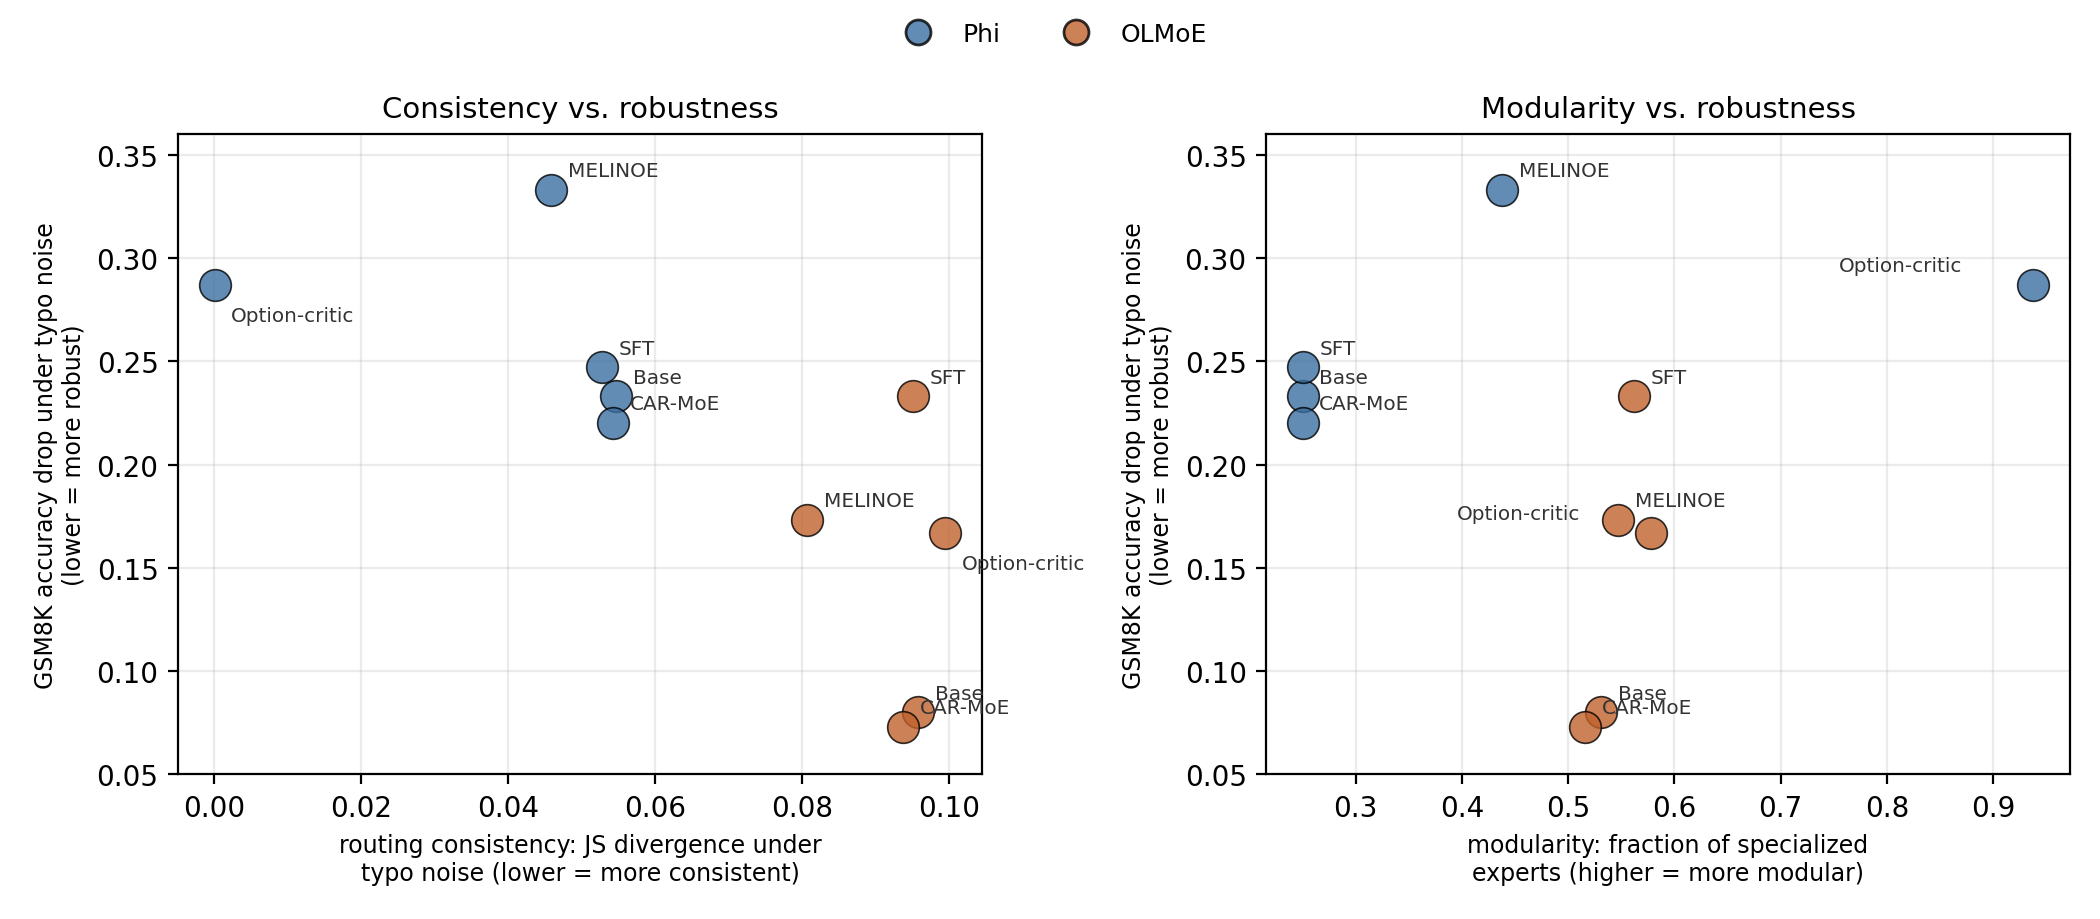
\includegraphics[width=\textwidth]{figures/consistency_modularity_robustness.png}
\caption{Left: consistency (JS divergence under typo noise) versus GSM8K accuracy drop
under the same perturbation. Right: modularity (fraction of specialized experts) versus
the same drop. CAR-MoE and Base/SFT cluster together within each backbone;
Phi-tiny-MoE's option-critic controller (labeled) is the outlier in both panels, maximally
consistent and "specialized," yet least robust.}
\label{fig:scatter}
\end{figure}

\section{Conclusion}

Routing consistency is not an end in itself; it is only useful evidence of modularity,
and modularity is only useful insofar as it makes a model robust to a changing
environment. Measuring benchmark performance, working-set efficiency, and
consistency/modularity statistics together, we found CAR-MoE the most robust objective on
both backbones, together with the best hit ratio and benchmark retention of any
non-collapsed objective, while an option-critic controller reached the best aggregate
consistency, specialization, and hit-ratio scores of any objective by collapsing its
routing entirely, paying for it with the worst downstream robustness. Future work in this
space should report a direct robustness check alongside any consistency or hit-ratio
metric, since the latter, alone,
cannot rule out this degenerate explanation.

\bibliographystyle{plainnat}
\begin{thebibliography}{99}

\bibitem[Shen and Henderson(2026)]{shen2026temporal}
Shen, Y. and Henderson, P.
\newblock Temporally Extended Mixture-of-Experts via Option-Critic.
\newblock \emph{arXiv preprint arXiv:2604.20156}, 2026.

\bibitem[Bacon et al.(2017)]{bacon2017optioncritic}
Bacon, P.-L., Harb, J., and Precup, D.
\newblock The Option-Critic Architecture.
\newblock \emph{Proceedings of the AAAI Conference on Artificial Intelligence}, 2017.

\bibitem[Raje et al.(2026)]{raje2026melinoe}
Raje, A., Nayak, A., and Joshi, A.
\newblock MELINOE: Fine-Tuning Mixture-of-Experts Language Models for Cache-Friendly Offloaded Inference.
\newblock \emph{arXiv preprint arXiv:2602.11192}, 2026.

\bibitem[Shao et al.(2024)]{shao2024deepseekmath}
Shao, Z., Wang, P., Zhu, Q., Xu, R., Song, J., Bi, X., Zhang, H., Zhang, M., Li, Y.~K., Wu, Y., and Guo, D.
\newblock DeepSeekMath: Pushing the Limits of Mathematical Reasoning in Open Language Models.
\newblock \emph{arXiv preprint arXiv:2402.03300}, 2024.

\bibitem[Yu et al.(2025)]{yu2025dapo}
Yu, Q., Zhang, Z., Zhu, R., Yuan, Y., Zuo, X., Yue, Y., Fan, T., Liu, G., Liu, L., Liu, X., et al.
\newblock DAPO: An Open-Source LLM Reinforcement Learning System at Scale.
\newblock \emph{arXiv preprint arXiv:2503.14476}, 2025.

\bibitem[NVIDIA(2025)]{nvidia2025nemotron}
NVIDIA.
\newblock Nemotron Post-Training Dataset v2.
\newblock \emph{Hugging Face Dataset Card}, 2025.

\bibitem[Lin(1991)]{lin1991divergence}
Lin, J.
\newblock Divergence Measures Based on the Shannon Entropy.
\newblock \emph{IEEE Transactions on Information Theory}, 37(1):145--151, 1991.

\bibitem[Belinkov and Bisk(2018)]{belinkov2018synthetic}
Belinkov, Y. and Bisk, Y.
\newblock Synthetic and Natural Noise Both Break Neural Machine Translation.
\newblock \emph{Proceedings of the International Conference on Learning Representations}, 2018.

\bibitem[Csord\'as et al.(2021)]{csordas2021modular}
Csord\'as, R., van Steenkiste, S., and Schmidhuber, J.
\newblock Are Neural Nets Modular? Inspecting Functional Modularity Through Differentiable Weight Masks.
\newblock \emph{Proceedings of the International Conference on Learning Representations}, 2021.

\end{thebibliography}

\appendix

\section{Experimental Setup Details}
\label{app:setup}

\paragraph{Backbones.} We evaluate two MoE backbones of different scale. Phi-tiny-MoE-
instruct has 32 transformer layers, 16 experts per MoE layer, top-2 routing, hidden size
4096, and expert intermediate size 448. OLMoE-1B-7B-0125-Instruct has 16 layers, 64
experts per layer, top-8 routing, hidden size 2048, and expert intermediate size 1024,
activating roughly 1B of its 7B total parameters per token. All objectives simulate the
working-set cache at the middle transformer layer of each backbone (layer 16 for
Phi-tiny-MoE, layer 8 for OLMoE-1B-7B), at a capacity fixed as a fraction of the total
expert count: $c=4$ (25\% of 16 experts) for Phi-tiny-MoE and $c=16$ (25\% of 64 experts)
for OLMoE-1B-7B.

\paragraph{Dataset.} Training and the consistency/modularity prompt pools are drawn from
the Nemotron Post-Training Dataset v2 \citep{nvidia2025nemotron}, a large instruction
dataset organized into topical splits; we use its \texttt{math} and \texttt{code} splits
throughout, sampled independently for the modularity comparison and jointly for the
consistency prompt pool. We filter rather than truncate: a candidate conversation is
scanned and tokenized, and dropped entirely if its prompt exceeds 1024 tokens (add all
messages up to but not including the model's turn, rendered through the backbone's own
chat template), rather than clipped to fit, so every prompt used at evaluation time is a
complete, untruncated conversation turn. We additionally require at least one assistant
turn present in the original conversation and reject rows with empty message content.
Prompts are sampled uniformly at random (reservoir sampling) from a per-split candidate
pool without replacement, with a fixed seed shared across every objective so all five
objectives per backbone see the identical prompt set. The consistency and modularity
measurements each use 256 prompts (512 total per domain-pair comparison for modularity,
since math and code are sampled independently at 256 each); the robustness measurement
uses 150 held-out GSM8K test questions, evaluated with a fixed four-shot prompt and
greedy decoding up to 256 new tokens, with answers extracted via a
\texttt{"\#\#\#\# <n>"} regex matching GSM8K's own answer format, no lm-eval-harness
dependency. The typo perturbation used throughout corrupts 5\% of alphabetic characters
per prompt (each corrupted character is replaced with a uniformly random lowercase letter
or deleted, with equal probability); the cosmetic perturbation used only for the
consistency measure randomly upper- or lower-cases 15\% of words and randomly duplicates
whitespace around 30\% of newlines, changing surface form without altering any character
identity within a word.

\section{Per-Expert Specialization Detail}
\label{app:spec}

Table~\ref{tab:main}'s specialization fraction is the share of experts with
$|P(\text{math}\mid e) - 0.5| \times 2 > 0.6$ out of $E$ total experts (16 for
Phi-tiny-MoE, 64 for OLMoE-1B-7B). The mean specialization index, not shown in the main
table for space, follows the same ordering as the fraction reported: Phi-tiny-MoE base
0.450, SFT 0.434, CAR-MoE 0.430, option-critic 0.938, MELINOE 0.533; OLMoE base 0.563,
SFT 0.612, CAR-MoE 0.567, option-critic 0.604, MELINOE 0.631. The cross-domain
Jensen-Shannon divergence between each objective's math- and code-domain expert usage
distributions, a complementary modularity signal where high values indicate the router
genuinely reroutes between domains rather than using a fixed subset regardless of
content, is: Phi-tiny-MoE base 0.159, SFT 0.138, CAR-MoE 0.149, option-critic 0.0001,
MELINOE 0.243; OLMoE base 0.128, SFT 0.150, CAR-MoE 0.128, option-critic 0.139, MELINOE
0.121. Notably, the option-critic controller's near-zero cross-domain divergence confirms
the collapse account directly: a router that used the same fixed experts regardless of
domain would show zero divergence between domains by construction, exactly what is
observed, whereas every other objective on either backbone shows a divergence at least
three orders of magnitude larger.

\section{Routing Trace: One Prompt, Base vs.\ CAR-MoE}
\label{app:trace}

Figure~\ref{fig:trace} shows the top-1 expert chosen at every generated token, at the
working-set layer, for a single held-out prompt under Phi-tiny-MoE's base model and under
CAR-MoE. The contrast is qualitative but stark: the base model's expert choice flickers
between many different experts almost every token, while CAR-MoE's choice organizes into
long contiguous runs of the same expert, the token-level signature of the working-set
reward's aggregate hit-ratio and cache-miss improvements reported in
Table~\ref{tab:main}.

\begin{figure}[h]
\centering
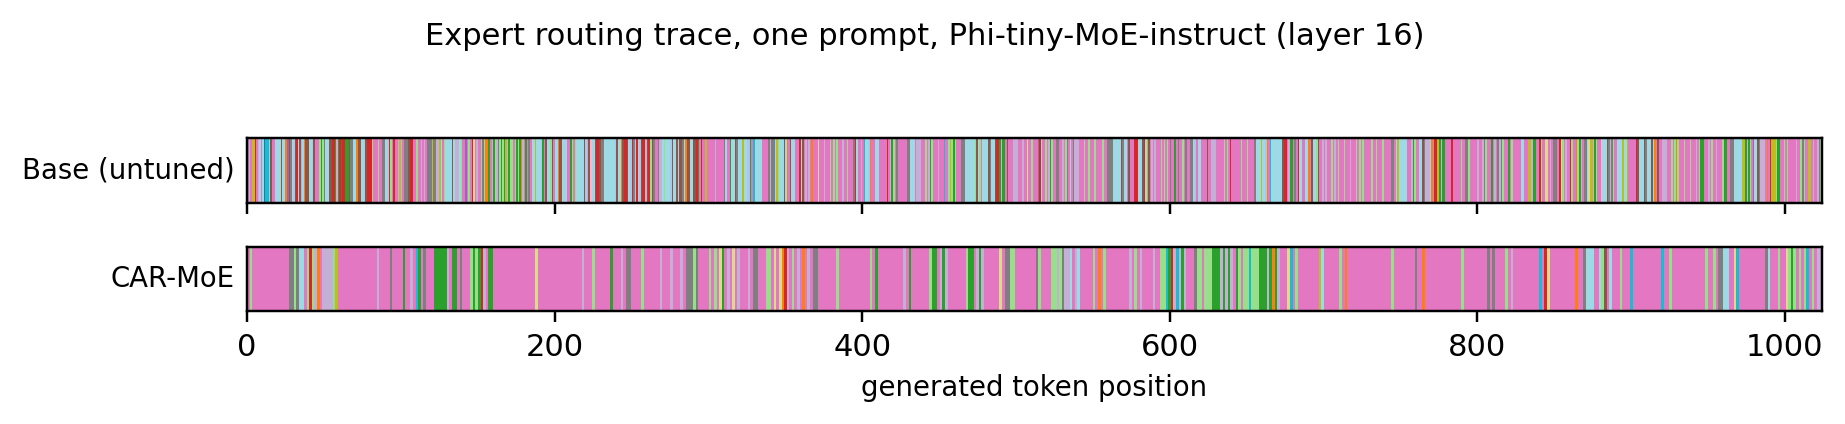
\includegraphics[width=\textwidth]{figures/trace_compare.png}
\caption{Top-1 expert id per generated token (color) at the working-set layer, for one
held-out prompt, Phi-tiny-MoE-instruct. Top: base model, routing switches almost every
token. Bottom: CAR-MoE, routing organizes into long contiguous same-expert segments.}
\label{fig:trace}
\end{figure}

\end{document}
